\documentclass[12pt]{article}
\usepackage[utf8]{inputenc}
\usepackage[T1]{fontenc}
\usepackage[francais]{babel}
\usepackage{layout}
\usepackage{geometry}
\usepackage{soul}
\usepackage{ulem}
\usepackage{url}
\usepackage{amsmath}
\usepackage{amssymb}
\usepackage{mathrsfs}
\usepackage{graphicx}
\usepackage{wrapfig}
\usepackage{tikz}
\usepackage{pgfplots}

\title{Présentation du projet de recherche : 
What's cooking ? Use recipe ingredients to categorize the cuisine
}
\author{Ayman \bsc{Hamzaoui} \& Julien \bsc{Delaunay}}
\date{\today} 
\pagestyle{plain}
\begin{document}
\maketitle
\newpage
\tableofcontents

\newpage
\section{Introduction}
Nous avons choisi la base de données \textit{"What's cooking ? Use recipe ingredients to categorize the cuisine"}\footnote{\url{https://www.kaggle.com/c/whats-cooking-kernels-only}} parmi les bases de données de Kaggle. Le domaine de cette base de données nous est apparu intéressant et nous avons remarqué que les données fournies semblent pouvoir être séparés et ainsi analysées avec les outils appris en cours.

\section{Les données}
Les données fournies par Kaggle sont sous la forme de deux documents json. Le fichier de test et le fichier d'entraînement. Pour le fichier d'entraînement, nous avons un id de la recette, le type de cuisine pour cette recette et les ingrédients nécessaires à sa fabrication. 

\begin{wrapfigure}[8]{r}{5cm}
	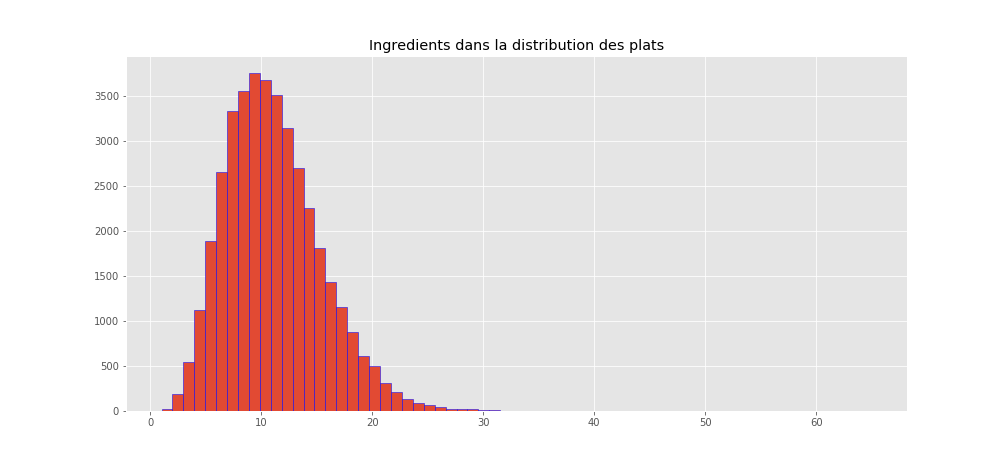
\includegraphics[width=4cm]{./repartitions_ingredients.png}
	\caption{Repartition des ingrédients}
	\label{label-image1}
\end{wrapfigure}
Nous avons effectué des recherches sur les données fournies afin d'obtenir quelques informations. Nous avons ainsi découvert que les cuisines utilisent entre 1 et 65 ingrédients par recette. Les ingrédients les plus utilisés varient en fonction des cuisines, il est donc intéressant d'observer si un modèle peut prévoir en fonction des ingrédients à quelle cuisine la recette appartient.

Nous avons observer que la base de données comportait 20 recettes, c'est donc un problème de classification avec des classes multiples. Il y a plus que 2 catégories à prédire.

\begin{wrapfigure}[5]{l}{6cm}
	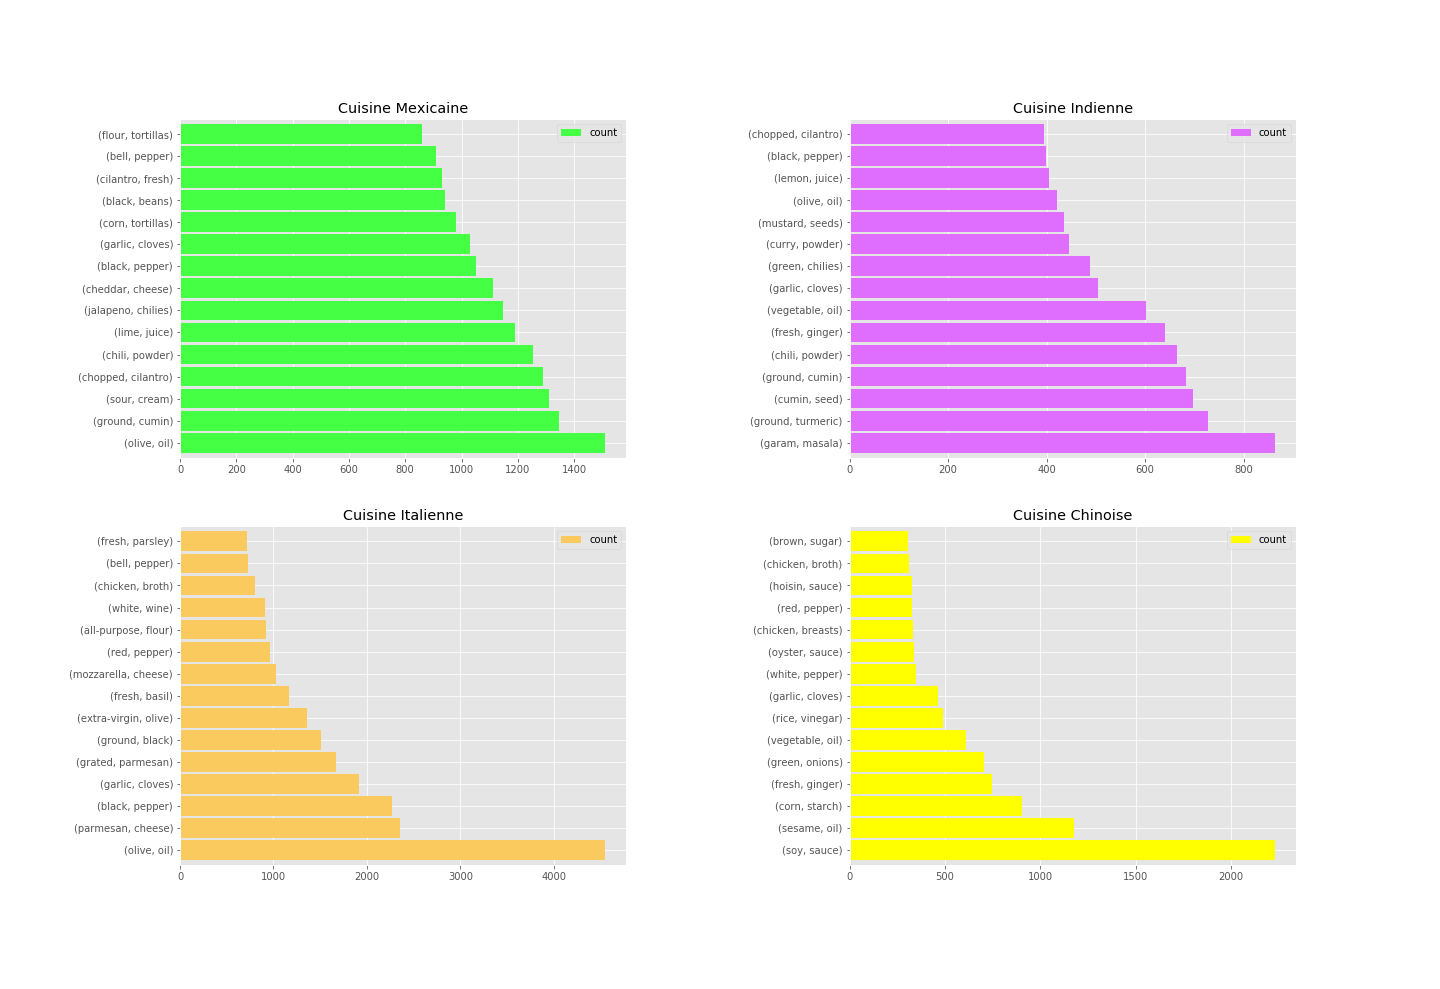
\includegraphics[width=6cm]{./exemple_differences_ingredients.png}
	\caption{Repartition des ingrédients par cuisine}
	\label{label-image2}
\end{wrapfigure}
Afin de commencer l'analyse et le traitement des données nous avons décidé de modifier le format d'entrée et transformer la liste des ingrédients sous la forme d'un tableau, avec une recette par ligne, et un ingrédients par colonne.

\newpage
\section{Les méthodes utilisées}
\subsection{TF-IDF}
\subsection{Methode 2}
\subsection{Methode 3}
\subsection{Methode 4}
\subsection{Methode 5}
\subsection{Methode 6}


\newpage
\section{Les résultats}


\section{Conclusion}



\newpage
\appendix
\section{Choix du design}
\begin{wrapfigure}[10]{r}{5cm}
	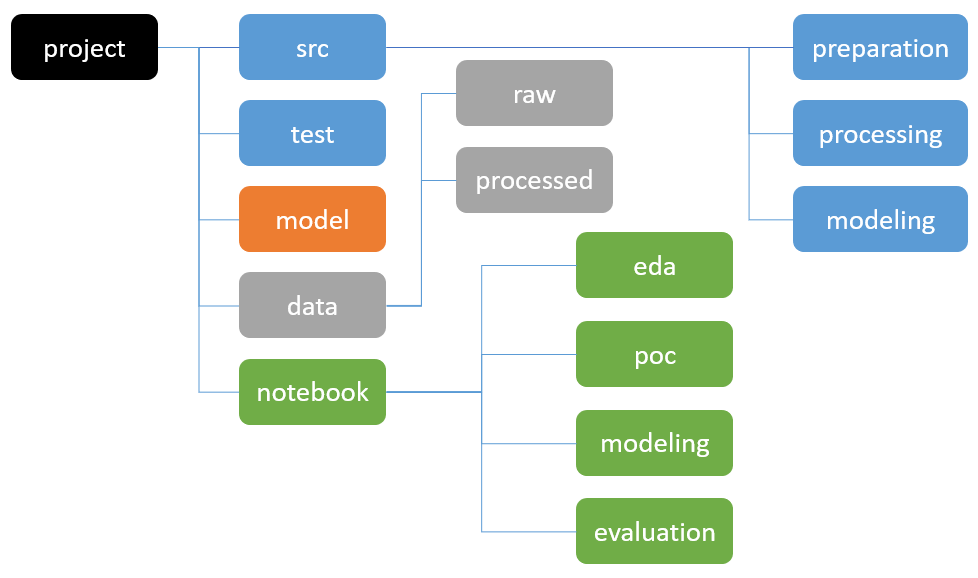
\includegraphics[width=4cm]{./projet_structure.png}
	\caption{Design d'un projet de Data Science}
\end{wrapfigure}
Pour le designe du code, nous avons utilisé ce format qui nous est inspiré de l'article écrit par Edward Ma\footnote{\url{https://goo.gl/a8cffw}}. Nous avons donc utiliser jupyter pour commencer à travailler sur les données afin de faciliter et rendre plus rapide le début du projet.


\section{Utilisation de Git}
Nous avons mis en place un github\footnote{\url{https://github.com/hamzaouiayman/IFT_712_projet_session.git}} afin de répartir le travail et indiquer le travail restant à faire. Pour cela, nous avons crée des \textit{issues}\footnote{Tâches à effectuer avant la fin du projet} au fur et à mesure de l'avancée du projet.

\end{document}